\section{Experimental Studies}

In Section~\ref{sec:unknowns} we described the concept of the unknown unknowns and in Section~\ref{sec:btm} we described a gamified structure that incentivizes humans to identify such unknown unknowns in a predictive model.

To provide a experimental evaluation of BTM, we asked two questions:
\begin{itemize}

\item Does BTM identify errors efficiently?

\item Does BTM identify isolated examples of unknown unknowns, or does it identify systematic unknown-unknown regions in the space?

\item Can we use the discovered errors to improve the models?

\end{itemize}

For our experiments, we used the BTM system to challenge two
classification systems. One for detecting pages with hate speech, and
one for detecting pages with adult content. We ran the systems with
the configuration details described in the previous section (0.2 cents
for the base task, 50 cents maximum payment for a URL that generates
an error).



\textbf{Comparison with stratified random examination:} 

In the application domain, the standard procedure for quality assurance of models
such as these is stratified random examination of model predictions.  
Examining a uniform random sample of the output is particularly uninformative, as the classifiers are quite accurate and the distributions are quite unbalanced, and so the vast majority of cases are correctly classified and not objectionable.  Therefore, standard procedure is to have human workers examine a random sample, stratified into bins by the model's confidence score.  Specifically, the range of confidence scores [0,1] was divided into $k$ equal-width bins.  A set of $N$ URLs for testing was sampled randomly, with $\frac{N}{k}$ from each bin.  This stratification is used because it generally finds more errors---it over-samples the URLs for which the models have low confidence (and are likely to be wrong).\footnote{It also allows the managment and data science teams to estimate the calibration of the scoring system, by examining the percentages of positive and negative instances in each bin.}  However, the discovered errors are likely to be ``known unknowns.''  

We compared this quality assurance procedure with BTM.  It is important not to see this as a bake-off.  Although we will compare identified error rates, the bottom line is that the two procedures are complementary: they are designed to assess different quantities.

For the adult classifier, the human workers in the stratified examination 
identified errors in 16\%
of the inspected cases---\textit{orders of magnitude} higher than the natural error
rate of the classifier.  In contrast, using BTM, more than 25\% of
the submitted cases exhibited an error. The
corresponding statistics for hate speech favored BTM even more
strongly: workers identified errors in only 9\% of the inspections for
stratified examination.  Workers identified errors in 27\% of the inspected
URLs with BTM.
On the surface, these results seem to indicate that the BTM process is
more efficient than the standard quality assurance procedure in identifying
problematic cases.  However, you may have noted that we could increase the
``efficiency'' of the non-BTM procedure by simply sampling a larger proportion from
the low-confidence predictions. 
Unfortunately, this would directly reduce the
number of ``unknown unknowns'' discovered.  At the extreme, the
largest number of errors would be found by sampling only in the
low-confidence region.  All the errors found would then be known
unknowns.  

% \foster{Insert a projection of the rate of finding UUs for (1) random sampling, and (2) if the stratification were all on the top bucket.  Add these estimations to the bar charts.}


\textbf{Comparing the severity of errors:} Figure~s\ref{fig:hate-speech} and~\ref{fig:adult} show the distribution of modeling mistakes identified for the hate speech and adult content tasks, respectively.  The blue bars show the mistakes identified by BTM; the red bars show the mistakes identified by the stratified evaluation.   The number ranges on the horizontal axis show the severity of the errors, in four buckets---how badly the classifier misjudged its classification.  The severities range from the least severe on the left (zero is no error), to maximum severity on the right: 1000 means that the classifier was certain of one class and the actual class was the other.  The unknown unknowns are on the far right of each graph.

A consistent behavior is observed for both categories: a significantly larger proportion of the BTM errors found are severe misses---the unknown unknowns. Within the errors identified by BTM, 25\% were cases of high severity; here the model was confident that it was making the correct decision (classifying the content as benign, with the highest confidence), but in reality the decision was incorrect. 

In sum, only does BTM identify a larger number of problematic predictions than the stratified testing, but also a significant number of these predictions were unknown unknowns.  These cases would be missed in practice and without an unpleasant event (possibly a catastrophe), we never would know that we had missed them. In contrast, and by now as expected, most of the identified 
errors for the stratified examination were misses that occur near the decision boundary.

\begin{figure}[t]
\centering
\center{
\subfigure[Hate Speech]{
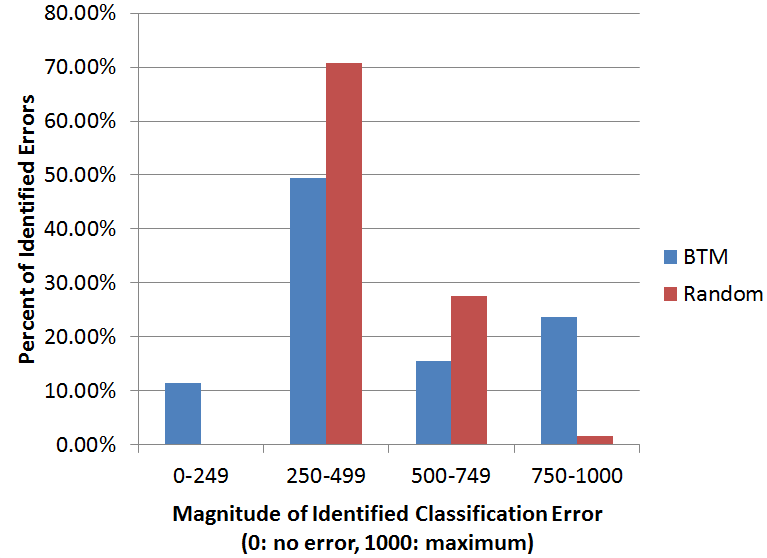
\includegraphics[width= 0.4\columnwidth]{plots/Hate-speech-scores.PNG}
\label{fig:hate-speech}
}
\subfigure[Adult Content]{
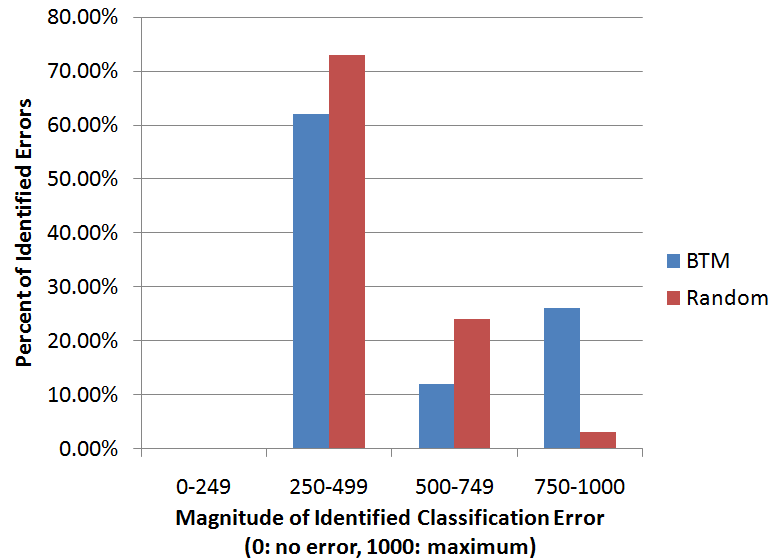
\includegraphics[width= 0.4 \columnwidth]{plots/porn-scores.PNG}
\label{fig:adult}
}
\caption{Distributions of the magnitude of the identified mistakes in the predictive model's output by BTM and by random sampling for two ad safety tasks.  Each bar indicates the percentage of successfully identified mistakes that reside in the associated score range.}
}
\label{fig:results}
\end{figure}

\drop{
\begin{figure}[t]
\center{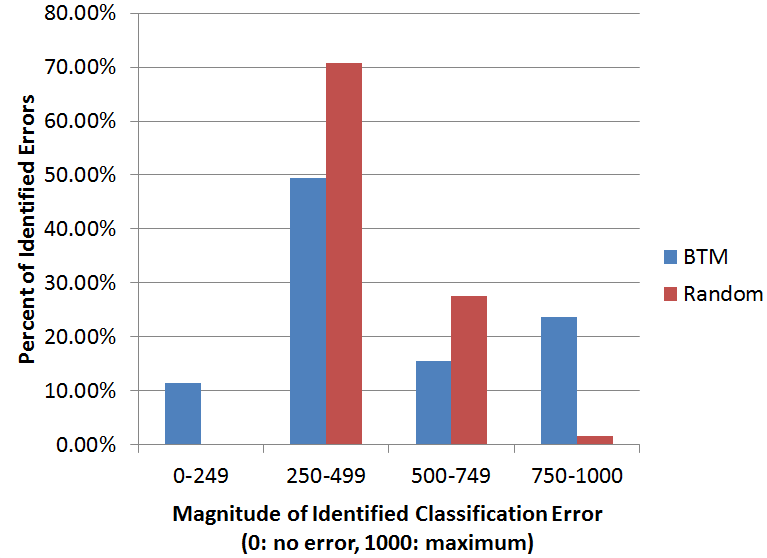
\includegraphics[width=0.4\columnwidth]{plots/Hate-speech-scores.PNG}}
\caption{A distribution of the magnitude of the identified errors by BTM and by random sampling for the hate speech category.}
\label{fig:hate-speech}
\end{figure}

\begin{figure}[t]
\center{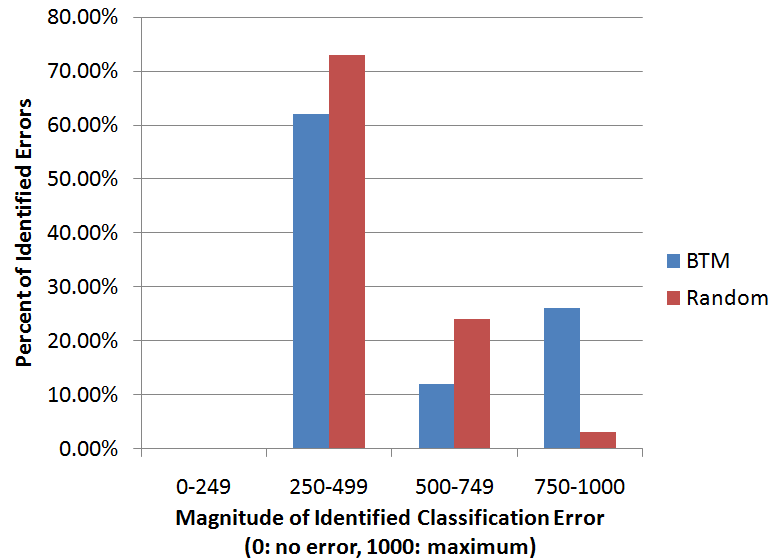
\includegraphics[width=0.4\columnwidth]{plots/porn-scores.PNG}}
\caption{A distribution of the magnitude of the identified errors by BTM and by random sampling for the adult content category.}
\label{fig:adult}
\end{figure}
}

\textbf{Isolated outliers or systematic regularities?}  A natural question to ask is if the cases found by BTM seem to be isolated outliers, or whether they seem to be regularities.  We framed this question pragmatically, based on the assumption that regularities can be modeled.\footnote{So therefore we may miss regularities that fall outside the limits of the inductive bias of our modeling procedures.} 

Following this reasoning, we ran the following experiment.  We attempted to learn a model that would classify positive and negative examples from amongst the BTM-identified cases.  Internal consistency in the identified errors would suggest that these cases are not outliers, but rather that they constitute parts of the space where the model fails systematically (potentially without being aware of the failures).
Figure~\ref{fig:curves} shows the results of this process. 

First consider the ``btm only'' learning curve and the ``student only'' learning curve, showing 10-fold cross-validated areas under the ROC curve (AUC).
The ``btm only'' curve shows the performance of models built and tested
using the error cases identified by the BTM process.  The ``student
only'' curve shows the performance of models built and tested using
examples gathered through stratified examination (the pages selected
by stratified examination were inspected by students for this
experiment, hence the name).  Importantly,
the results show that the quality of both models is fairly high.  This
illustrates that there is consistency and internal coherence in these
sets of identifed errors.  The fact that the BTM model can reach high levels of
accuracy indicates that BTM indeed identifies systematic regions that
contain unknown unknowns, and not just disparate outliers.  However,
note the difference between the quality that is achievable by training
with the two different data sets.  The comparatively lower quality of
the stratified examination model illustrates that these pages are inherently
more difficult to learn from; this is consistent with our discussion
above that the discovery via stratified random examination (DVSRE)
focuses on the ambiguous cases (those that the current model is
uncertain about), while BTM discovers incorrectly classified areas of
the space that have been systematically ignored.

We also can examine whether the two approaches (DVSRE and BTM) identify sets of similar examples, or whether each of them identifies something completely different. For that, we tested the performance of BTM-trained models using the examples from DVSRE (``student'') and vice versa. The results indicate that there is little cross-consistency between the models. What we discover using BTM has little effectiveness for classifying the error cases identified through DVSRE, and vice versa. This finding indicates that BTM and DVSRE reveals errors in different parts of the space; importantly, BTM finds errors that are systematically different from those found by DVSRE.
BTM and DVSRE are different processes, capable of identifying different types of errors. Each of these has its place in the evaluation and improvement of automatic models. DVSRE identifies primarily cases where the model already knows that it is not confident. 
The results show that even if the DVSRE were stratified only on the ``unknown'' region, it still would not identify nearly as many unknown unknowns as Beat the Machine.



\begin{figure}[t]
\center{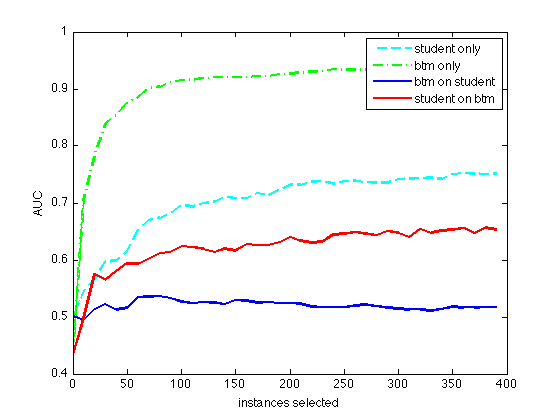
\includegraphics[width=0.6\columnwidth, height=2in]{plots/adt_btm_eval.png}}
\caption{Learning curves generated by the models
using cross-validation (BTM and student lines), and then use as test case for BTM the errors identified by random sampling (BTM on students), and vice versa (students on BTM).}
\label{fig:curves}
\end{figure}


